%SOP Template 
% Version 02 Added revision date
% Version 03 Added TOC and acknowledgements
%           New SOP3_alpha.cls


\documentclass[12pt]{../SOP3_alpha}

\usepackage[english]{babel}
\usepackage{blindtext}
\usepackage{lipsum}

\usepackage[version=4]{mhchem} 
\usepackage{pdfpages}

\title{Texture Analysis using a Hydrometer}
\date{7/12/2015}
\author{Marc Los Huertos \& Isaac Medina}
\approved{Los Huertos}
\ReviseDate{\today}
\SOPno{32 v0.1}

\usepackage{Sweave}
\begin{document}
\Sconcordance{concordance:Texture-Analysis-Using-Hydrometer_v01.tex:Texture-Analysis-Using-Hydrometer_v01.Rnw:%
1 22 1 1 0 294 1 6 0 1 5 31 1}


\maketitle

\section{Scope and Application}

\NP The size of soil particles plays a central role in soil process including soil-water-plant relations, pollution fate and transport, and nutrient cycling. In addition, soil texture classes have important land use implications, where, for example farmers, prefer loam soils to soils that are dominated by clays or sand.

\NP The applications implements D422 ASTM Method D422 to analyze soil sample with a hydrometer.

\section{Summary of Method}

\NP This SOP does this...

\tableofcontents

\newpage

\section{Acknowledgements}

\section{Definitions}

\NP Effective Diameter

\NP Texture Class...


\section{Biases and Interferences}

\NP The following are parameters that might influence the results of the hydrometer test and thus, we use various methods to pre-treat soils or measure to correct for these sources of bias. When correction factors are required, the calculations can become confusing.	 But we'll try to lead ourselves through this thicket without too many wrong-turns. 

\begin{description}
	\item[Temperature and Viscosity] Water temperate influences the viscosity of water, such that colder temperatures increase viscosity which increases the resistance force and reduces the terminal velocity of particles. The viscosity can be corrected for temperature.
	\item[Temperature and Density] The density of water is highest at 4.94 degrees C. As temperatures increases, the density of water decreases. As water density decreases, the suspension density $\rho_s$ decreases, thus the particle size distribution is not accurate without a correction. 
	\item[Soil Weight and Hygroscopic Water] Soil is composed of many components, including minerals, water, organic matter, air, etc. But to calculate the soil particle analysis, we need to account for the water in soil. We can do this by measuring the soil moisture content and correct the mass contributed by water from the soil tested.
	\item[Aggregated Soil Particles] Soil particles need to be dispersed, but there is no perfect way to accomplish this. Complete dispersion requires both mechanical and chemical assistance. Mechanical stirring overcomes weaker binding forces in large aggregates, but chemical agents are also necessary, especially to deflocculate clays. Polyvalent cations (normally \ce{Ca+2} and \ce{Al+3}) flocculate clays by forming interparticle, electrostatic links. Chemical dispersing agents (such as sodium hexametaphosphate) are effective in dispersing these clay bundles because:
	
	\begin{itemize}
		\item The sodium monovalent cation (\ce{Na+}) replaces polyvalent cations adsorbed on clays, breaking the interparticle linkage. The displaced polyvalent cations form insoluble complexes with phosphorus that prevents re-establishment of floccules.
		\item The adsorption of sodium, a highly hydrated cation, inducing the hydration of clays. This condition diminishes the binding strength between clay and cation which raises a clay particle's electronegativity and, hence, their repulsion from other clays.
	\end{itemize}
	
\noindent The mixture of dispersed soil particles in water is called a suspension. Once a true suspension state has been achieved, differential settling rates can be used to distinguish particle size distribution.
	
	\item Hydrometers are designed to be read from the bottom of the meniscus. However, in a soil suspension, the water is cloudy and we it's impossible to see through the meniscus. Therefore, we read the scale at the top of the meniscus and apply a correction factor. Without this correction factor, the analysis will be incorrect. 
\end{description}


\section{Health and Safety}

\NP Sodium hexametaphosphate is a non-hazardous material but may be irritating to skin and eyes. Dust may be irritating to lungs if inhaled. 

\subsection*{Safety and Personnnel Protective Equipment}

\NP Care should be taken to avoid inhalation. Handle powdered HMP in a well-ventilated area or fume hood. Chemical-safety goggles should be worn while pouring HMP solution and during blending to avoid contact with eyes. In case of contact, flush eyes with cold water for 15 minutes. Latex gloves should be worn to avoid contact with skin. Hands and contaminated skin should be washed thoroughly with soap and water after handling. Sweep, vacuum, scoop or remove spilled sodium hexametaphosphate. Flush residual area with water. In case of spills on clothes, wash thoroughly before wearing again. See the SDS for more information on contamination and spills.

\section{Personnel \& Training Responsibilities}

\NP Researchers training is required before this the procedures in this method can be used... 

\NP Researchers using this SOP should be trained for the following SOPs:

\begin{itemize}
  \item SOP01 Laboratory Safety
  \item SOP02 Field Safety
  \item SOP03 Handling Hardous Materials
\end{itemize}

\section{Required Materials and Apparati}

\begin{enumerate*}
	\item Sieve No. 10 and No. 200.
	\item 250-ml and 400-ml beakers
	\item Hot plate
	\item Soil tins
	\item Drying oven
	\item Milkshake Mixer and Dispersion Cup (metal milkshake cup)	
	\item 151H Hydrometer
	\item 1 L Sedimentation Cylinder and No. 13 stopper 
	\item Stopwatch
	\item Balance sensitive to 0.01 g for weighing the material passing sieves.
\end{enumerate*}

\section{Reagents and Standards}

\begin{enumerate*}
	\item Hydrogen peroxide, 30\%.
	\item Hydrochloric acid, 1N.
	\item Sodium hexametaphosphate
\end{enumerate*}

\section{Estimated Time}

\NP This procedure requires several days to complete.

\begin{table}
\begin{tabular}{llll}\hline
Task          & Time          & Elapsed Time  & Time until completion \\ \hline\hline
Collect Soil  & 1-3 hours     & 1-3 hours     &         \\ \hline
\end{tabular}
\end{table}

\section{Sample Collection, Preservation, and Storage}



\section{Procedure}

\NP Before beginning, we need to organize the procedures by day, since we can't complete the analysis during a single lab period.

\begin{description}
	\item[Session 1:] Air dry 200 grams of soil (could require more than one day);
	\item[Session 2:] Pass air-dry soils through No. 10 sieve; dry sub-sample for moisture content; 
	\item[Session 3:] Calculate and weigh $SW_e$ for pretreatment and/or dispersion; 
	\item[Session 4:] Conduct hydrometer measurements; and
	\item[Session 5:] Analyze particles retained on No. 200 sieve and complete data entry.
\end{description}

\subsection{Air-Dried Soil}

\NP After collecting a soil, we allow them to air dry by putting them in a tin or beaker and let them equalibrate with the laboratory for 24 or more hours. If the soils are very wet, this may take several days. 

\subsection{Determining Proportion of Soil Passing No. 10 Sieve}

\NP Soils are defined as particles that are less than 2 mm. Thus, we begin by removing the gravel, particles that exceed the sand-sized particles, >2.0 mm. These particles, however, influence the soil texture, so we will quantify the contribution of particles that exceed 2 mm. 

\NP We can do this by analyzing the soil that can pass through the No. 10 sieve, which has a mesh size of 2 mm.  

\begin{enumerate}
	\item Homogenize the soil by removing it from the bag and mix thoroughly;
	\item Weigh out approximately 65 g of silt or clay soils or 120 g of a sandy soil, record the value in Box 10. 
	\item Prepare soil with air-drying and pulverizing to pass a No. 10 mesh sieve (< 2 mm)-- pick out the rocks and use a mortar and pestle to break up the soil so that it all passes through the sieve. 
	\item Weigh the soil that passed through the sieve and record the weight in Box 11.
\end{enumerate}
  
\subsection{Measuring and Correcting for Soil Water Content}

\NP We will use air-dried soil for our test. However, even air-dried soil contains water. This moisture is associated with clay particles, salts, and organic matter and is often referred to as hygroscopic water. To calculate the soil moisture content, we weigh the soil before and after oven drying the soil at 110$^\circ$ C. Once we determine the moisture content, we can use the moisture content to correct for the water in the air-dried soil. Because this method relies on the change in soil mass, the water content is often referred to as gravimeter water content as opposed to a volumetric water content.

\NP This temperature is somewhat arbitrary, and clay minerals in particular may contain 10-15\% water (dry basis) at 400$^\circ$ C (Gardner 1986).  As temperature increases, first water in soil pores evaporates, then water adsorbed to mineral surfaces, followed by water between lattice layers and that which forms part of the mineral lattice itself.  The exact quantities and patterns of release in a hetergeneous mixture like soil depends on the particular mix of minerals making up a sample.  Water adsorbed to organic components (as well as other volatile organic substances) will also evaporate over a range of temperatures.  The key point is to specify the temperature used when reporting moisture data.

\NP To determine the hygroscopic water content,

\begin{enumerate}
	\item Weigh and record the weight of a soil tin (Appendix A, Box 13) and the tin \# (Appendix A, Box 12);
	\item Remove a 10-15 gram sub-sample from the air-dried soil that passed through the No. 10 sieve, put the sub-sample into the pre-weighed soil tin and record the weight (Appendix, Box 14);
	\item Dry the sample in a drying oven set at 110 $^\circ$ C for approximately 24 hours;
	\item Allow the tins to cool and record the oven-dried weight (Appendix, Box 15). 
\end{enumerate}

\NP We calculate the  hygroscopic moisture content we subtract the mass of oven-dried sample and the air-dried mass before drying, usually less than one, unless there is no hygroscopic moisture, then is is one. Use the following equation to calculate the water content

\begin{equation}
\texttt{Moisture}_H = (\texttt{air-dry mass w/tin} - \texttt{oven-dried mass w/tin})/(\texttt{air-dried mass} - \texttt{tin mass})
\end{equation}

\noindent $Moisture_H$ can be calculated using R code developed for this SOP. See Appendix B for a user guide for the program. 

\subsection{Calculating Soil Sample Mass}

\NP We then calculate the ``Total Sample Represented'' in the hydrometer test as the mass of soil in hydrometer test as the oven dry mass used by the percent passed through 2 mm sieve and multiply by 100.

\NP We will analyze air dried soil -- that has passed through a No. 10 sieve. 

\begin{equation}
W = oven dry mass * percent passing 2mm sieve * 100
\end{equation}

\begin{equation}
WB = \frac{M_{air}*10000}{Per_{No.10} * (100 + Moisture_H)}
\end{equation}

\NP But since the sample has hygroscopic water, we will use the correction factor above to weigh a ``oven-dried equivalent'', $DW_e$. 

\NP If the soils are coarse textured (>70\% sand), will will use $DW_e$ of 100 g, otherwise 50 g is sufficient.

\NP Since air dried soil contains water, the soil sample used will weigh slightly more than 50g or 100 g for sandy soils where $DW_e = DW_{air} * (1 + DW_c)$,\footnote{I need to check this!}, thus we can re-arrange the equation to determine the amount of air-dried soil to use for our test:

\begin{equation}
DW_{air} = 50/(1+DW_c)
\end{equation}

\noindent and for sandy soils,

\begin{equation}
DW_{air} = 100/(1+DW_c)
\end{equation}

\subsection*{Pre-Treatment}

\NP Soils should be pre-treatmented for soil high in organic matter \ldots

\begin{enumerate}
	\item Transfer 50 or 100 grams of dry weight equivalent ($DW_e$) grams of soil to a 400-ml glass beaker.
	
	\item Removal of carbonates: Add 50 mL DI water and sufficient 1 M \ce{HCl} to reduce the soil pH to between 3.0 and 4.0. Stir and allow to equilibrate 10 minutes until there is no effervescence.

	\item Removal of organic matter:\footnote{may need the previous treatment to wet and acidify the soil before this is done. Not clear.} Carefully add 10 ml of 30\% hydrogen peroxide (\ce{H2O2}), a few milliliters at a time, allowing effervescence to subside before adding more, until no more frothing occurs. If necessary, make the suspension acidic to litmus paper with a few drops of 1N HCl.  Oxidation with \ce{H2O2} requires an acidic medium. When frothing subsides heat to 90 $^\circ$C and add \ce{H2O2} until frothing subsides. Rinse down walls of beaker and continue heating until no excess \ce{H2O2} is consumed.

	\item Removal of iron oxides 
	%\citep[pp. 574-576]{kunze1986pretreatment}: 
	Add 150 mL of citrate-bicarbonate buffer to sample in beaker. Add 3 g of sodium hydrosulfite (\ce{Na2S2O3}) gradually as samples may froth.  Place in water bath at 80$^\circ$C for 20 minutes.  Place the blender cup on electrical mixer and stir for 10 minutes.

	\item Removal of soluble salts: Place soil in centrifuge tube and add 100 mL water and centrifuge for 10 min at 1500 rpm until supernatant is clear.  If the centrifuge is not clear, repeat the process until it is clear.

\end{enumerate}
 
\subsection*{Dispersing Soil Sample}

\begin{enumerate}
	\item Using the datasheet and the R function (\texttt{SoilEquiv()}) or web app (http://) to calculate $DW_e$;
	\item Weigh approximately $DW_e$g of soil (From Box 18) into the dispersion cup and record to the nearest 0.1gram (Box 6). 
	\item Record the dispersion cup number (Box 6).
	\item Add 125 mL of sodium hexametaphoshate (40 g/L). Stir so the slurry is thoroughly wetted. Cover and allow to soak for at least 16 hours. 
	\item Add distilled water up to the first ``indentation'' of the dispersion cup.
	\item Attach the dispersion cup to the mixer; mix 5 minutes for sandy soils, 15 minutes for fine-textured soils.
	
\end{enumerate}

\subsection{Conducting Hydrometer Tests}

\begin{enumerate}

	\item Make up a blank cylinder with 125 mL of sodium hexa-metaphosphate and add distilled water to the 1000 mL mark.  Record the blank hydrometer reading and temperature. If the reading is above 0 (zero) on the hydrometer scale (in other words, if the zero mark is below the surface), record the blank correction as a negative number.  Read at the top of the meniscus.
	
	\item Transfer soil suspension to sedimentation cylinder; use distilled water from squirt bottle to get all of sample from mixing cup.

	\item Fill cylinder to 1000-mL mark with distilled water.

	\item Cover the cylinder with a stopper (No. 13) and invert the cylinder 180 degrees for a full minute, where the cylinder should be turned upside-down and back should take 2 seconds. You may need to vigorously mix the cylinder for the first two turns to loosen the soil at the bottom.
	
	\item After the minute of inverting, begin timing.  While slowing spinning the hydrometer remove air bubbles, carefully lower the hydrometer into suspension after 20s; record the hydrometer reading at 40 seconds. Remove the hydrometer and rinse the hydrometer between each reading. 
	
	\item This 40-second reading should be \textbf{repeated to obtain 3 accurate} after repeating the inversion process. Because the suspension is opaque, read the hydrometer at the top of the meniscus rather than at the bottom. There is a correction for this!

	\item After final 40-second reading, remove hydrometer, carefully lower a thermometer into the suspension and record the temperature (degrees C).  Mixing raises temperature by 3-5$^\circ$C, so it is important to record the temperature for both hydrometer readings (See Table \ref{tab:ReadingTimes}).
	
		\item The hydrometer must be removed and rinsed and dried after each reading. If this is not followed, the hydrometer will be accumulate particles on the glass walls and become increasingly inaccurate. 

	\item Take a hydrometer reading at the following times:
	
		\begin{table}
		\begin{tabular}{lrrr}\hline
Obs. & Soil Reading Times 		& Temperture		& Blank Hydrometer \\ \hline\hline	
0		& Before Inverting (0 seconds)		&	 X	&		X		\\
1		& 40 seconds (Repeat twice) 			&	 		&			  \\
2		&	2.0 minutes 										&			&       \\
3		&	5.0 minutes 										&	 X 	&		X   \\
4		&	15 minutes 											&	 		&   	  \\
5	 	& 30 minutes 											&			&				\\
6		& 60 minutes 											&		X	& 	X		\\
%X		& 90 minutes 										&			&				\\
7		& 2	hours													& 	X	& 	X		\\
8		& 3 hours (optional)							&		X	& 	X		\\
9   & 6 or 8 hours (optional)					&		X	& 	X		\\
10		& 24 hours											&		X	&  	X 	\\\hline		
		\end{tabular}
		\caption{Reading times modified from \textbf{citet{standard2007d422}}. These times can be adjusted, be sure to record the actual times in Boxes 19 and 20.}
		\label{tab:ReadingTimes}
	\end{table}
	
	\item Be sure that the cylinder is back from the edge of the counter and in a location where it won't be disturbed.	
	
\end{enumerate}

\subsection*{Determining Proportion of Soil Retained No. 200 Sieve}

\NP Particles retained on the No. 200 sieve are larger are often categorized as sand. As the hydrometer does very little to distinshin between size fractionation of sand -- very fine, fine, medium, course, and very course sand. 

\NP But collecting the particles on the No. 200 sieve, we can use seives to better understand the soil characteristics. We can do this by analyzing the mass of the soils retained on the No. 200 sieve, which has a mesh size of XX 0.125 mm.  

\begin{enumerate}
	\item Poor the contents of the cylinder through a No. 200 sieve;
	\item Using the sink with a sediment trap, wash the soil in the sieve until the water leaving the sieve is clear. 
	\item Select a soil tin, and record the tin \# (Box XX) and tin mass (Box XX). 
	\item Carefully wash the soil from the tin into the soil, without damaging the sieve screen. The screens are quite delicate, so using a squeeze bottle is probably best. Using a brush or metal device will force particles into the screen, which can get stuck, distort and stretch the mesh openings or otherwise damage them. 
	\item Weigh the dry soil with the soil tin and record the results in Box Xx.
\end{enumerate}

\section{Recording the Results}

Record the results in Appendix A, Then enter the data into the data entry form (\href{test}{http\\:test}. Other columns calculations will be produced with the R code from Appendix B.  


\section{Data Analysis and Calculations}

Once the data has been entered in the online form, you can extract the data as a csv file. This csv file can then be called by R to calculate the data automatically, using the following functions. 

\subsection*{Importing Data}

Import and check data integrity

\begin{Schunk}
\begin{Sinput}
> #hydrometer = import()
> #head(hydrometer)
> #str(hydrometer)
\end{Sinput}
\end{Schunk}

What should you be looking for?  We want to make sure the data shown are the same as expected. There are several ways to look at the data to determine this. I have shown two ways. 1) Looking at the header (first six observations), then we evaluate the structure of the dataframe.
 
\subsection{Calculating effective diameter, $D_e$}


\subsection{Calculating the Percent Finer, PF}


\subsection{Graphing and Interpreting the Results}

\section{QC/QA Criteria}

\section{References}

\NP D422...

\NP Wilde, S.A., R.B. Corey, J.G. Iyer, and G.K. Voigt.  1979.  Soil and Plant Analysis for Tree Culture.  Oxford and IBH Publishing Co., New Delhi.  Pp. 12-13.

\NP Anderson, J.M., and J.S. Ingram, eds.  1993.  Tropical Soil Biology and Fertility:  A Handbook of Methods. 2nd ed.  CAB International, Wallingford, UK.  P. 93-94.

\section{Appendix A. Data Sheet}

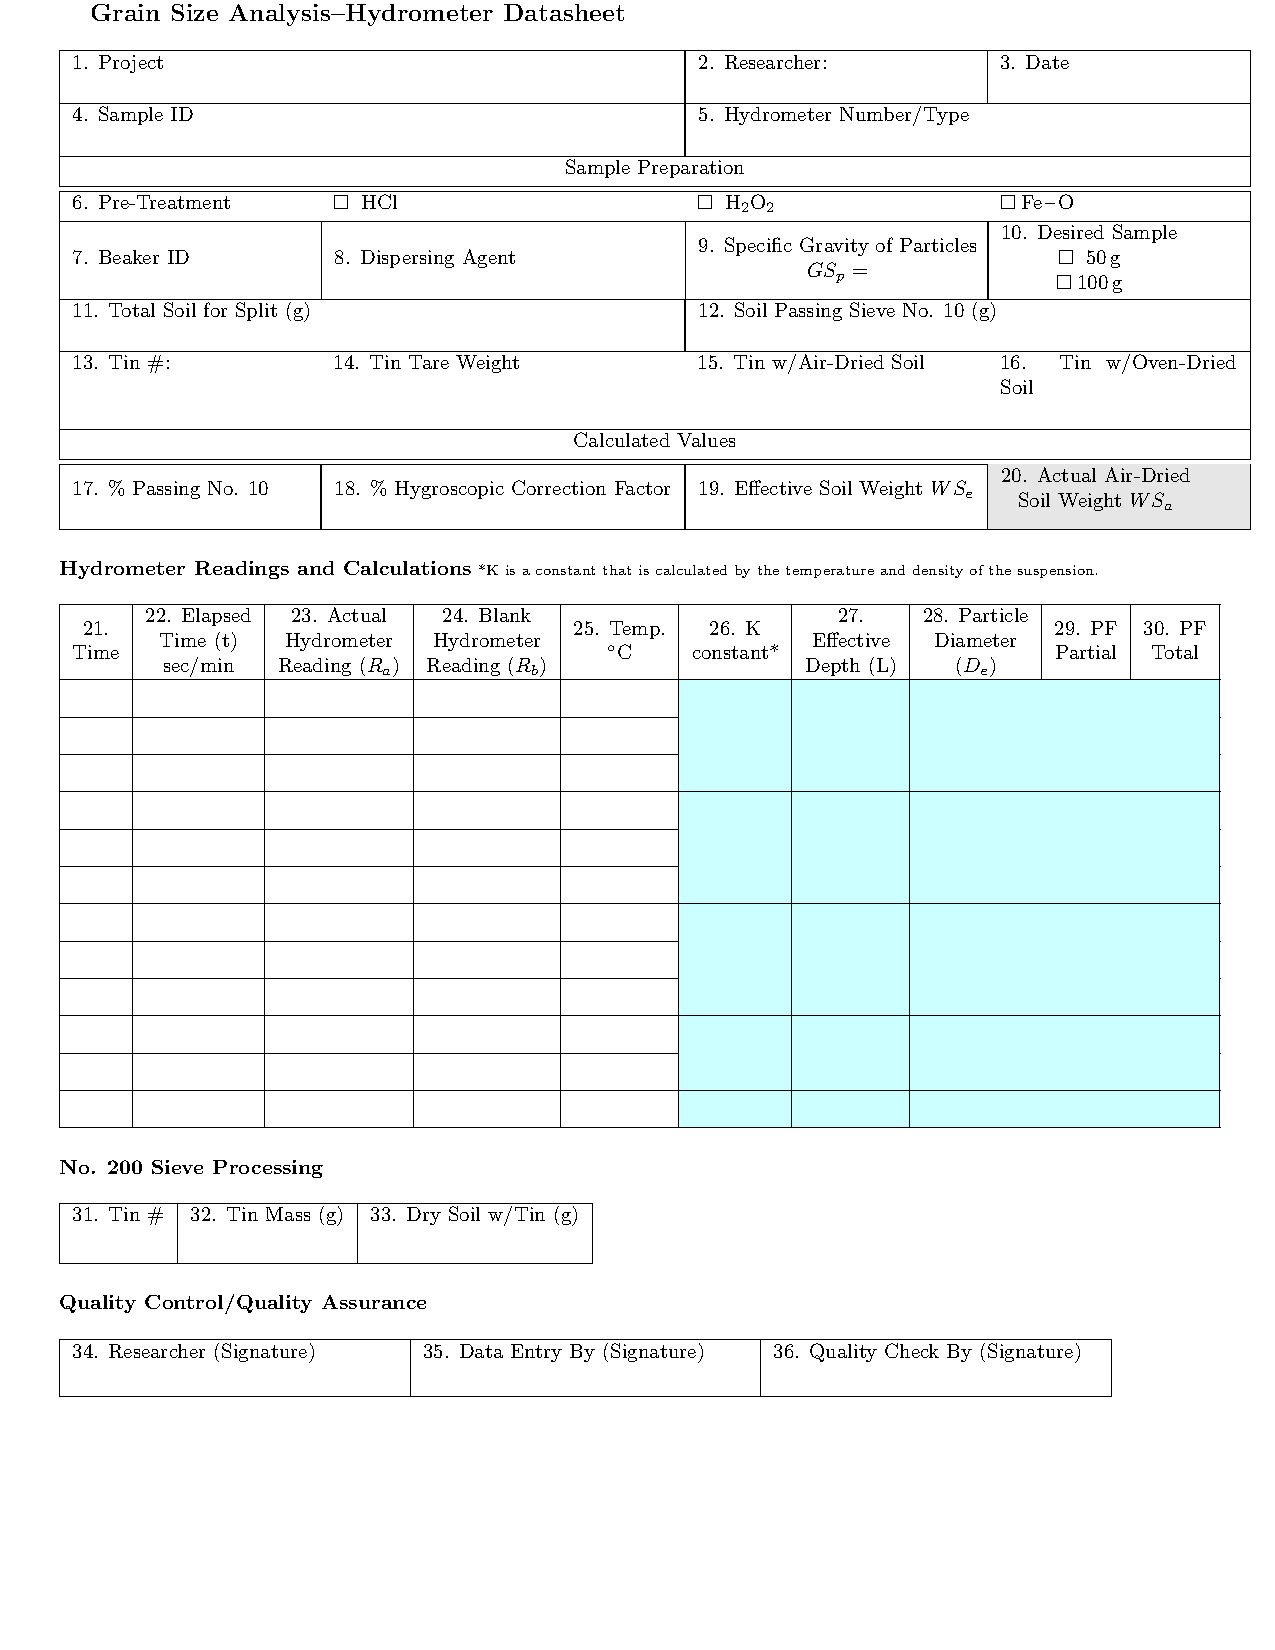
\includepdf[pages=-]{DataSheetv3}


\newpage
\section{Appendix B: R code to calculate parameters for the SOP}

% \input{Appendix B}	

\end{document}
